\documentclass[a4paper,12pt]{article}
\usepackage{amssymb}
\usepackage{amsmath}
\usepackage{xcolor,color}
\usepackage{tikz}
\usetikzlibrary{shapes.geometric,positioning,decorations.pathreplacing,decorations.pathmorphing,patterns,decorations.markings}
\usetikzlibrary{arrows.meta}

\begin{document}

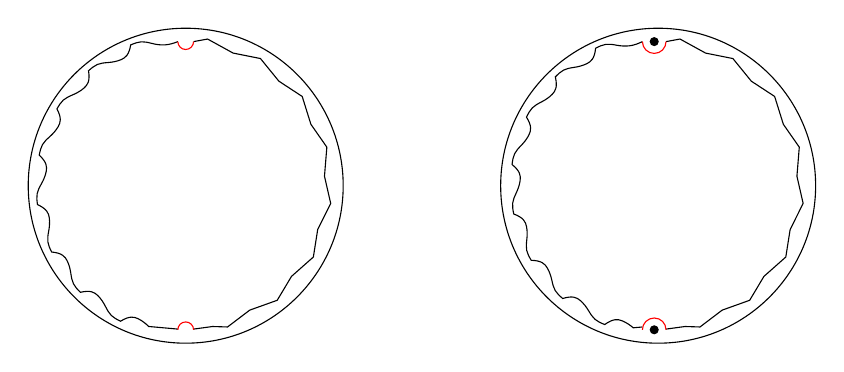
\begin{tikzpicture}[scale=1]
\draw
(2,2) arc (0:360:2); \draw[%red,
decoration={coil,segment length=6mm,amplitude=0.3mm},decorate] (-0.1,3.83) arc (94:266:1.83);
\draw[%red,
decoration={zigzag,
segment length=7mm,amplitude=0.45mm},decorate] (0.1,3.83) arc (86:-86:1.83);
\draw[red] (-0.1,3.83)%
arc (180:360:0.1);
\draw[red] (-0.1,0.17) arc (180:0:0.1);
\draw
(8,2) arc (0:360:2); \draw[%red,
decoration={coil,segment length=6mm,amplitude=0.3mm},decorate] (5.8,3.83) arc (98:262:1.83);
\draw[%red,
decoration={zigzag,
segment length=7mm,amplitude=0.45mm},decorate] (6.1,3.83) arc (86:-86:1.83);
\draw[red] (5.8,3.83)%
arc (180:360:0.15);
\draw[red] (5.8,0.17) arc (180:0:0.15);
\draw[fill=black] (5.95,3.83) circle (0.05cm);
\draw[fill=black] (5.95,0.17) circle (0.05cm);
\end{tikzpicture}

\end{document}